\documentclass[11pt,twocolumn]{article}
\usepackage{enumerate}
\usepackage[hidelinks]{hyperref}
\usepackage{amsmath, amssymb, textcomp}
\usepackage{graphicx}
\usepackage[section]{placeins}
\usepackage{cite}
\usepackage{color}

\begin{document}

\title{The Ising model\\ {\large Computational Physics}}
\author{Tobias de Jong\\ s0881260}
\date{\today} % Voeg automatisch de datum in

\maketitle
\newcommand{\Part}[3][ ]{\ensuremath{\frac{\partial^{#1} #2}{{\partial #3}^{#1}}}}
\newcommand{\Dif}[3][ ]{\ensuremath{\frac{d^{#1} #2}{{d #3}^{#1}}}}
\renewcommand{\O}[1]{\ensuremath{\mathcal{O}\left(#1\right)}}
\renewcommand{\vec}{\bold}
\section{Introduction}
In this paper we will investigate the different properties of the Ising model in 2D and 3D using Monte Carlo simulation methods. The canonical Metropolis single spin flip method as well as the Wolff cluster flip algorithm are used to obtain values for the critical exponents $\chi$, $\gamma$ and $\nu$ in both 2D and 3D. %for different lattices
\section{Theory}
\subsection{Ising model}
\subsection{Monte Carlo approximation}
\section{Algorithms}
\subsection{Metropolis}
The Metropolis algorithm~\cite{Metropolis} utilizes single spin flips to transition between states. By selecting a random spin at each step we make sure that the transition chance  between any two neighbouring states $\mu$, $\nu$ is equal:
\[g(\mu,\nu) = g(\mu,\nu) = \frac1N\]
\subsection{Wolff}
The Metropolis algorithm has as major disadvantage that the thermalization slows down exponentially around the critical point. As this is the area in parameter space we are most interested in, another algorithm is needed. We use an algorithm proposed by Wolff in 1989~\cite{Wolff}. In essence, this algorithm stochastically builds up a cluster which it will flip at once, thus negating the critical slowdown.
\section{Implementation}
Both the Metropolis and the Wolff algorithm were implemented using Python and NumPy. While this choice of language will not result in the fastest implementation it yields easily readable and adaptable code. 
Moreover, simple libraries exist to parallelise the different runs to keep the total wall clock computation time reasonable.
The other major benefit of using python is of course easy access to extensive plotting libraries.
\section{Results}
\subsection{Thermalization \& Auto-correlation}
To visualize the thermalization we do several runs for each value of $\beta$, calculate the magnetisation for each and take the mean across different runs. This way, the plot will be a flat line at the equilibrium value when thermalized. Results for a $40\times40$ grid and 100 runs per value of beta is given in figure \ref{therm}. The obvious conclusion here is that the thermalisation time depends quite strongly on $\beta$, especially around the critical point, which constitutes the interesting part of the data. An algorithm which would bypass this slow-down behaviour would thus be beneficial. As mentioned, the Wolff algorithm is such an algorithm, as although it still needs to thermalize, the thermalization time does not diverge around the critical point.
\begin{figure}[!ht]
\centering 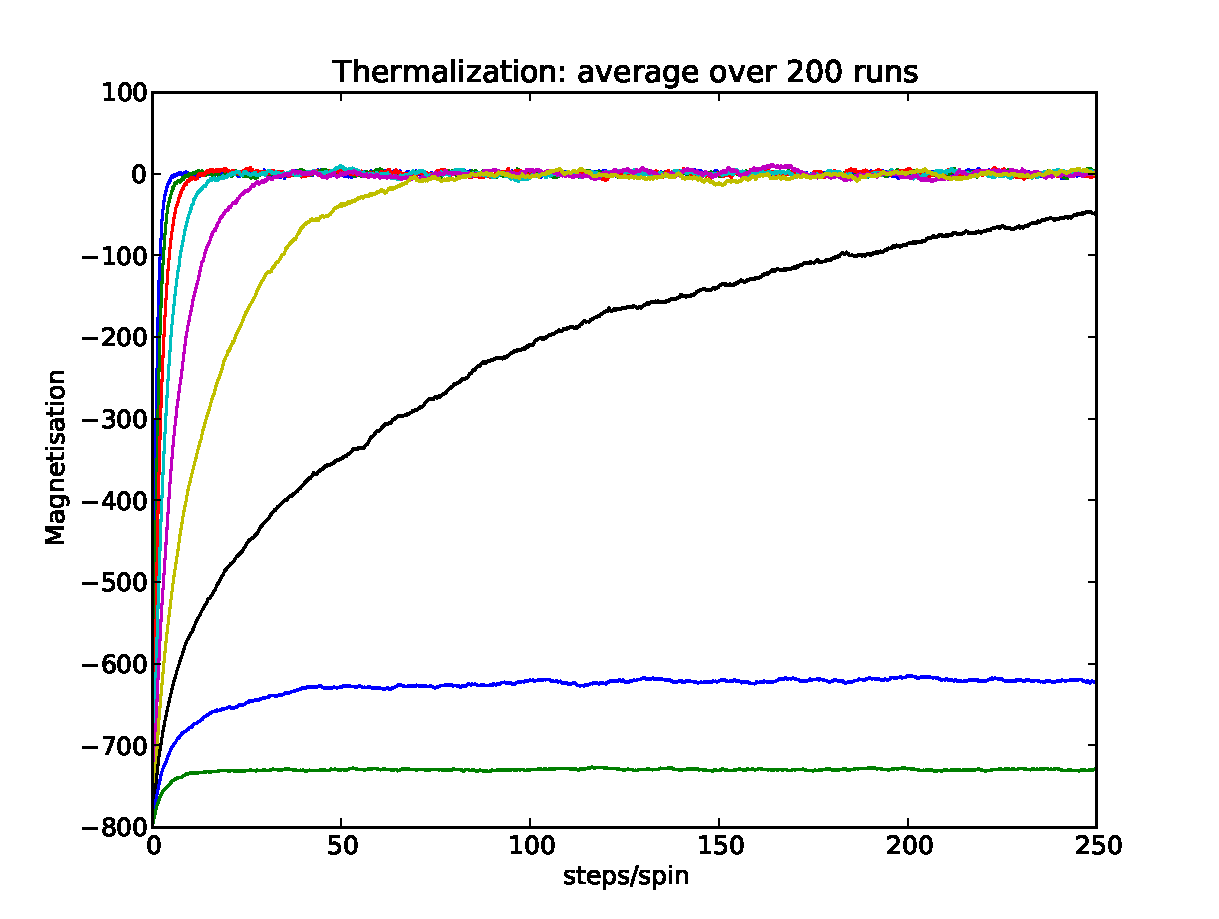
\includegraphics[width=\columnwidth]{figs/therm.pdf}
\caption{Thermalization}
\label{therm}
\end{figure}
The normalized autocorrelation of the Magnetisation and the energy for diverse values of $\beta J$ is given in figures \ref{magcorrel} and \ref{Ecorrel}.
\subsection{Finite size scaling}
\section{Data collapse}
\subsection{Rectangular 2D lattice}
To obtain a data collapse we use the values as found by Newman and Barkema \cite{Thebook}: $\gamma = 1.76$, $\nu = 1.00$ and $T_c=2.269J$. For the exponent $\beta$ we used the exact value $\frac18$. The result is shown in figure \ref{2Dcollapse}. Shuffling with the zoomed dataset gives the best collapse for $T_c = 2.271$, $\beta =0.139$, $\nu =0.997$, $\gamma =1.76$.
\subsection{Hexagonal 2d lattice}
To check the universality of the critical exponents we also ran the simulations for a hexagonal lattice. All values are kept the same as compared to the previous section, except for $T_c$, which we starting with the critical exponents found for the rectangular lattice. This yields $T_c=3.6378$. The result can be seen in figure \ref{Hexcollapse}.
\subsection{3 dimensions}
To estimate the values of the critical exponents for 3 dimensions, we use Wolff's algorithm to run for lattice sizes of $10^3$, $20^3$ and $30^3$ spins, both in rectangular and hexagonal close packing lattices. We use the first $10^3$ run of both lattices to estimate the critical temperature and adjust the range of simulated temperatures closer around the critical point, to keep computation time wihin reasonable boundaries.\\
An attempt at a data collapse is then visually attempted, by varying the critical exponents and -temperature until the curves best overlap. The resulting plot for a rectangular lattice is shown in \ref{collapse3Drect}, the resulting one for the hcp-lattice in figure \ref{collapse3Dhcp}. Note that due to the higher coordination number the critical temperature is shifted, but the critical exponents are the same.
\bibliography{verslag}{}
\bibliographystyle{plain}


\end{document}
